%%
%% Class homework & solution template for latex
%% Alex Ihler
%%
\documentclass[twoside,11pt]{article}
\usepackage{amsmath,amsfonts,amssymb,amsthm}
\usepackage{graphicx,color}
\usepackage{verbatim,url}
\usepackage{listings}
\usepackage{upquote}
\usepackage[T1]{fontenc}
%\usepackage{lmodern}
\usepackage[scaled]{beramono}
\usepackage{enumerate}
\usepackage{float}
%\usepackage{textcomp}

% Directories for other source files and images
\newcommand{\bibtexdir}{../bib}
\newcommand{\figdir}{figs}

\newcommand{\E}{\mathrm{E}}
\newcommand{\Var}{\mathrm{Var}}
\newcommand{\N}{\mathcal{N}}
\newcommand{\matlab}{{\sc Matlab}\ }

\setlength{\textheight}{9in} \setlength{\textwidth}{6.5in}
\setlength{\oddsidemargin}{-.25in}  % Centers text.
\setlength{\evensidemargin}{-.25in} %
\setlength{\topmargin}{0in} %
\setlength{\headheight}{0in} %
\setlength{\headsep}{0in} %

\renewcommand{\labelenumi}{(\alph{enumi})}
\renewcommand{\labelenumii}{(\arabic{enumii})}

\theoremstyle{definition}
\newtheorem{MatEx}{M{\scriptsize{ATLAB}} Usage Example}

\definecolor{comments}{rgb}{0,.5,0}
\definecolor{backgnd}{rgb}{.95,.95,.95}
\definecolor{string}{rgb}{.2,.2,.2}
\lstset{language=Matlab}
\lstset{basicstyle=\small\ttfamily,
        mathescape=true,
        emptylines=1, showlines=true,
        backgroundcolor=\color{backgnd},
        commentstyle=\color{comments}\ttfamily, %\rmfamily,
        stringstyle=\color{string}\ttfamily,
        keywordstyle=\ttfamily, %\normalfont,
        showstringspaces=false}
\newcommand{\matp}{\mathbf{\gg}}




\begin{document}

\centerline{\Large Kyle Benson}
\centerline{CS 273A - Machine Learning: Fall 2013}
\centerline{Homework 2}

% % % % % % % % % % % % % % % % % % % % % % % % % % % % % % % % % % % % % % % % % % % % % % % % % % % % %
\subsection*{Problem 1: Bayes Classifiers}

\begin{enumerate}[(a)]
\item Probabilities for Naive Bayes Classifier: \\
$p(y=1) = 0.4$ \\
\begin{tabular}{|c|c|c|c|c|c|c|}\hline
$p(Variable = 1 | y = 1)$ & $x_1$ & $x_2$ & $x_3$ & $x_4$ & $x_5$ & $\prod$ \\
\hline
Probability & 0.75 & 0.0 & 0.75 & 0.5 & 0.25 & 0 \\
\hline
$p(Variable = 1 | y = -1)$ & $x_1$ & $x_2$ & $x_3$ & $x_4$ & $x_5$ & $\prod$ \\
\hline
Probability & 0.5 & 0.833 & 0.667 & 0.833 & 0.33 & .0756\\
\hline
\end{tabular}

\item For $x=(00000), p(y=1)\prod\limits_{i}p(x_i=0) = 0.4 * (0.25*1*0.25*0.5*0.75) = 0.009375$
and $p(y=-1)\prod\limits_{i}p(x_i=0) = 0.6 * (0.5*0.167*0.33*0.167*0.67) = 0.00185$.
So the predicted class would be $y=1$ 

For $x=(11010), p(y=1)\prod\limits_{i}p(X_i=x_i) = 0.4 * (0.75 * 1 * 0.25 * 0.5 * 0.75) = 0.028$
and $p(y=-1)\prod\limits_{i}p(x_i=0) = 0.6 * (0.5 * 0.833 * 0.333 * 0.833 * 0.667) = 0.046236114$.
So the predicted class would be $y=-1$

\item $p(y=1 | x = (1 1 0 1 0)) = 
\frac{p(y=1)p(x=(1 1 0 1 0) | y=1)}{p(x=(1 1 0 1 0))} =
\frac{0.4 * (0.75 * 1 * 0.25 * 0.5 * 0.75)}
{(0.75 * 1 * 0.25 * 0.5 * 0.75) + (0.5 * 0.833 * 0.333 * 0.833 * 0.667)}
= 0.0087
$

\item Because then our probability table will have $O(F^2)$, rather than $O(F)$, entries, where $F$ is the number of features we are training on,
in order to account for dependence among the feature variables.

\item We do not need to re-train the model.  Because $x_1$ is independent of all other $x_i$, we can safely ignore $x_1$ entirely and make our predictions based on the classifier: $p(y)\prod\limits_{i\neq1}x_i$
\end{enumerate}

% % % % % % % % % % % % % % % % % % % % % % % % % % % % % % % % % % % % % % % % % % % % % % % % % % % % % % % % % % % % % % % %

\subsection*{Problem 2: Decision Trees}

\begin{enumerate}[(a)]

\item $H(y) = - 0.4 * log(0.4) - 0.6*log(0.6) = 0.971$

\item Using the formula $H(y|x_i = 0) = p(y=1 | x_i = 0) \log p(y=1 | x_i = 0) + p(y=0 | x_i = 0) \log p(y=0 | x_i = 0)$
\begin{tabular}{|c|c|c|c|c|c|}\hline
$Variable$ & $x_1$ & $x_2$ & $x_3$ & $x_4$ & $x_5$ \\
\hline
Entropy $H(y|x_i = 0)$ & 1 & 0.4312 & 1.03 & 0.931 & 0.887 \\
\hline
Entropy $H(y|x_i = 1)$ & 0.811 & 0.22 & 0.701 & 0.72 & 1.028 \\
\hline
Info Gain & 0.0465 & 0.61 & 0.006 & 0.0914 & 0.006 \\
\hline
\end{tabular}
\\ Therefore, we should split on feature $x_?$ first.

%\item 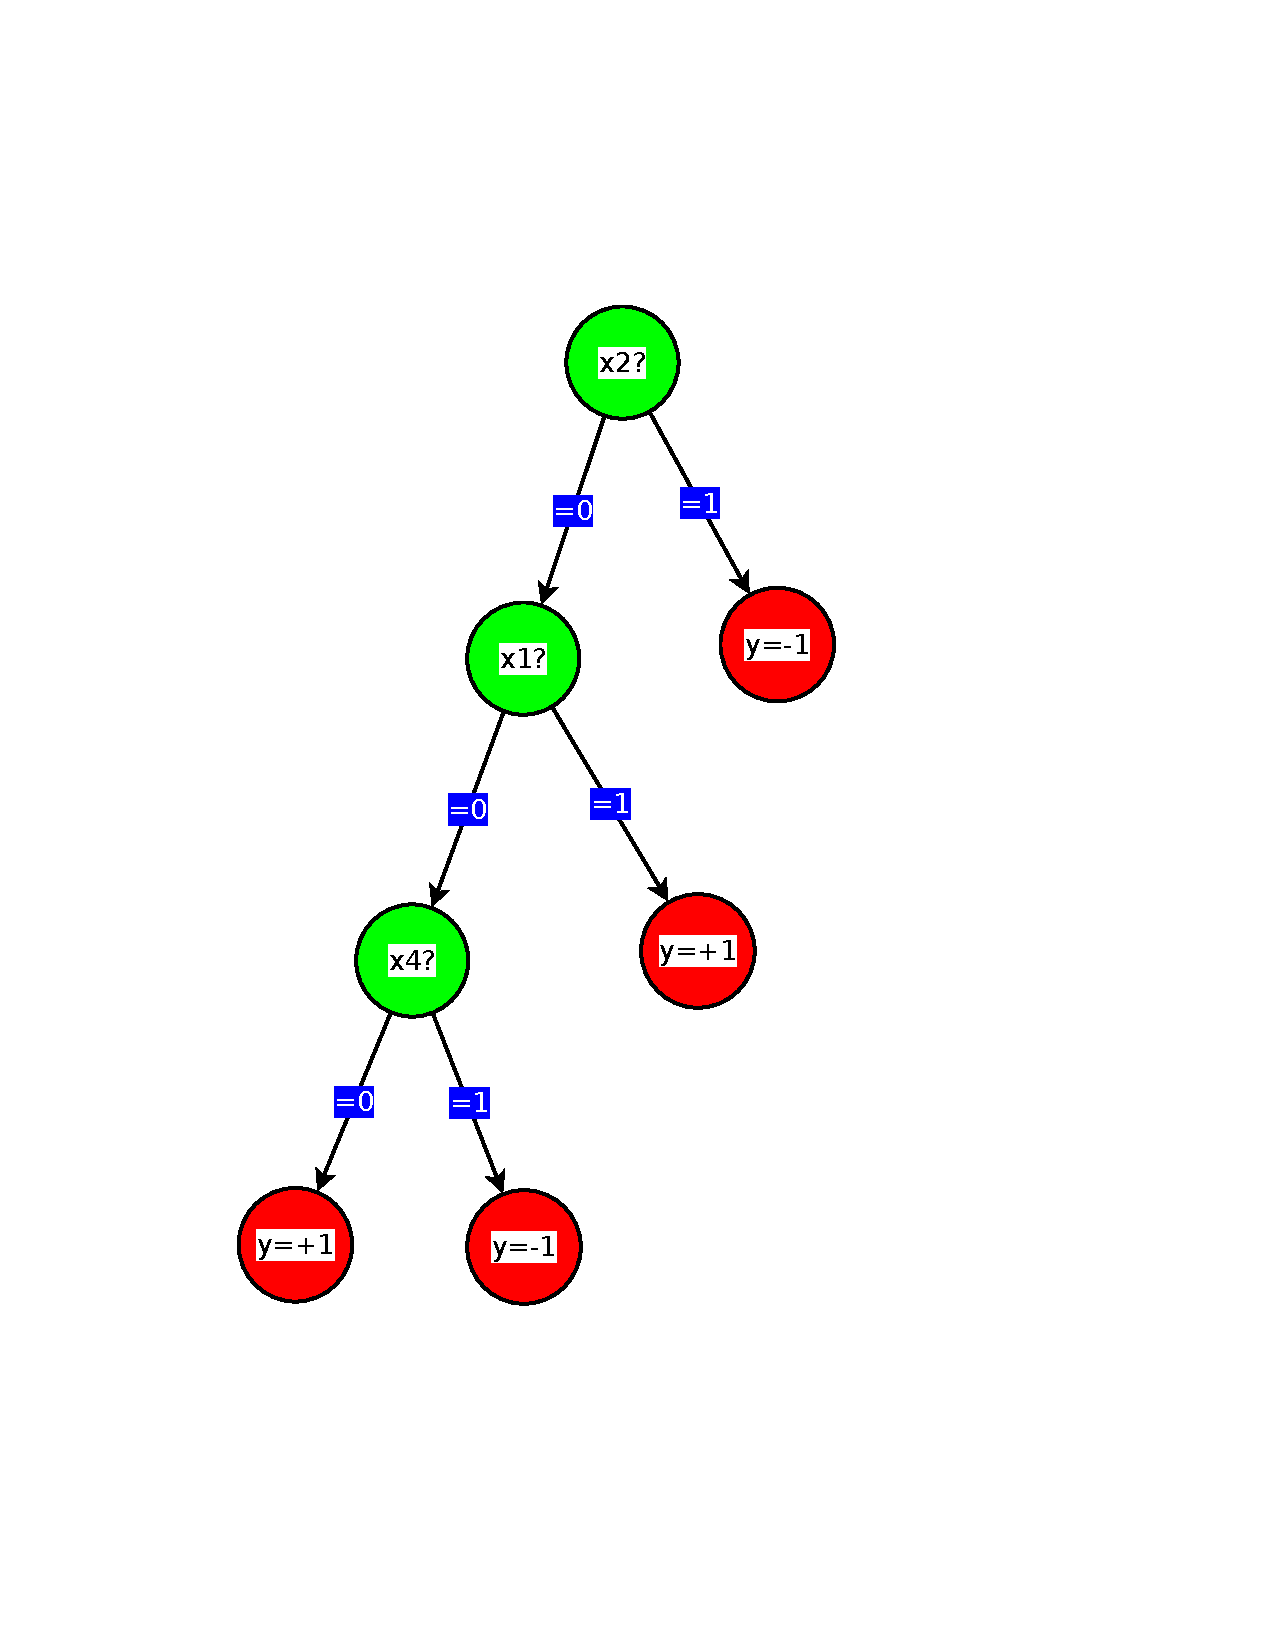
\includegraphics{problem2_tree}
\end{enumerate}

% % % % % % % % % % % % % % % % % % % % % % % % % % % % % % % % % % % % % % % % % % % % % % % % % % % % % % % % % % % % % % % %

\subsection*{Problem 2: K-Nearest Neighbors and Validation}

\begin{enumerate}[(a)]
\item 
\begin{figure}[H] \centering
\begin{tabular}{cccc}
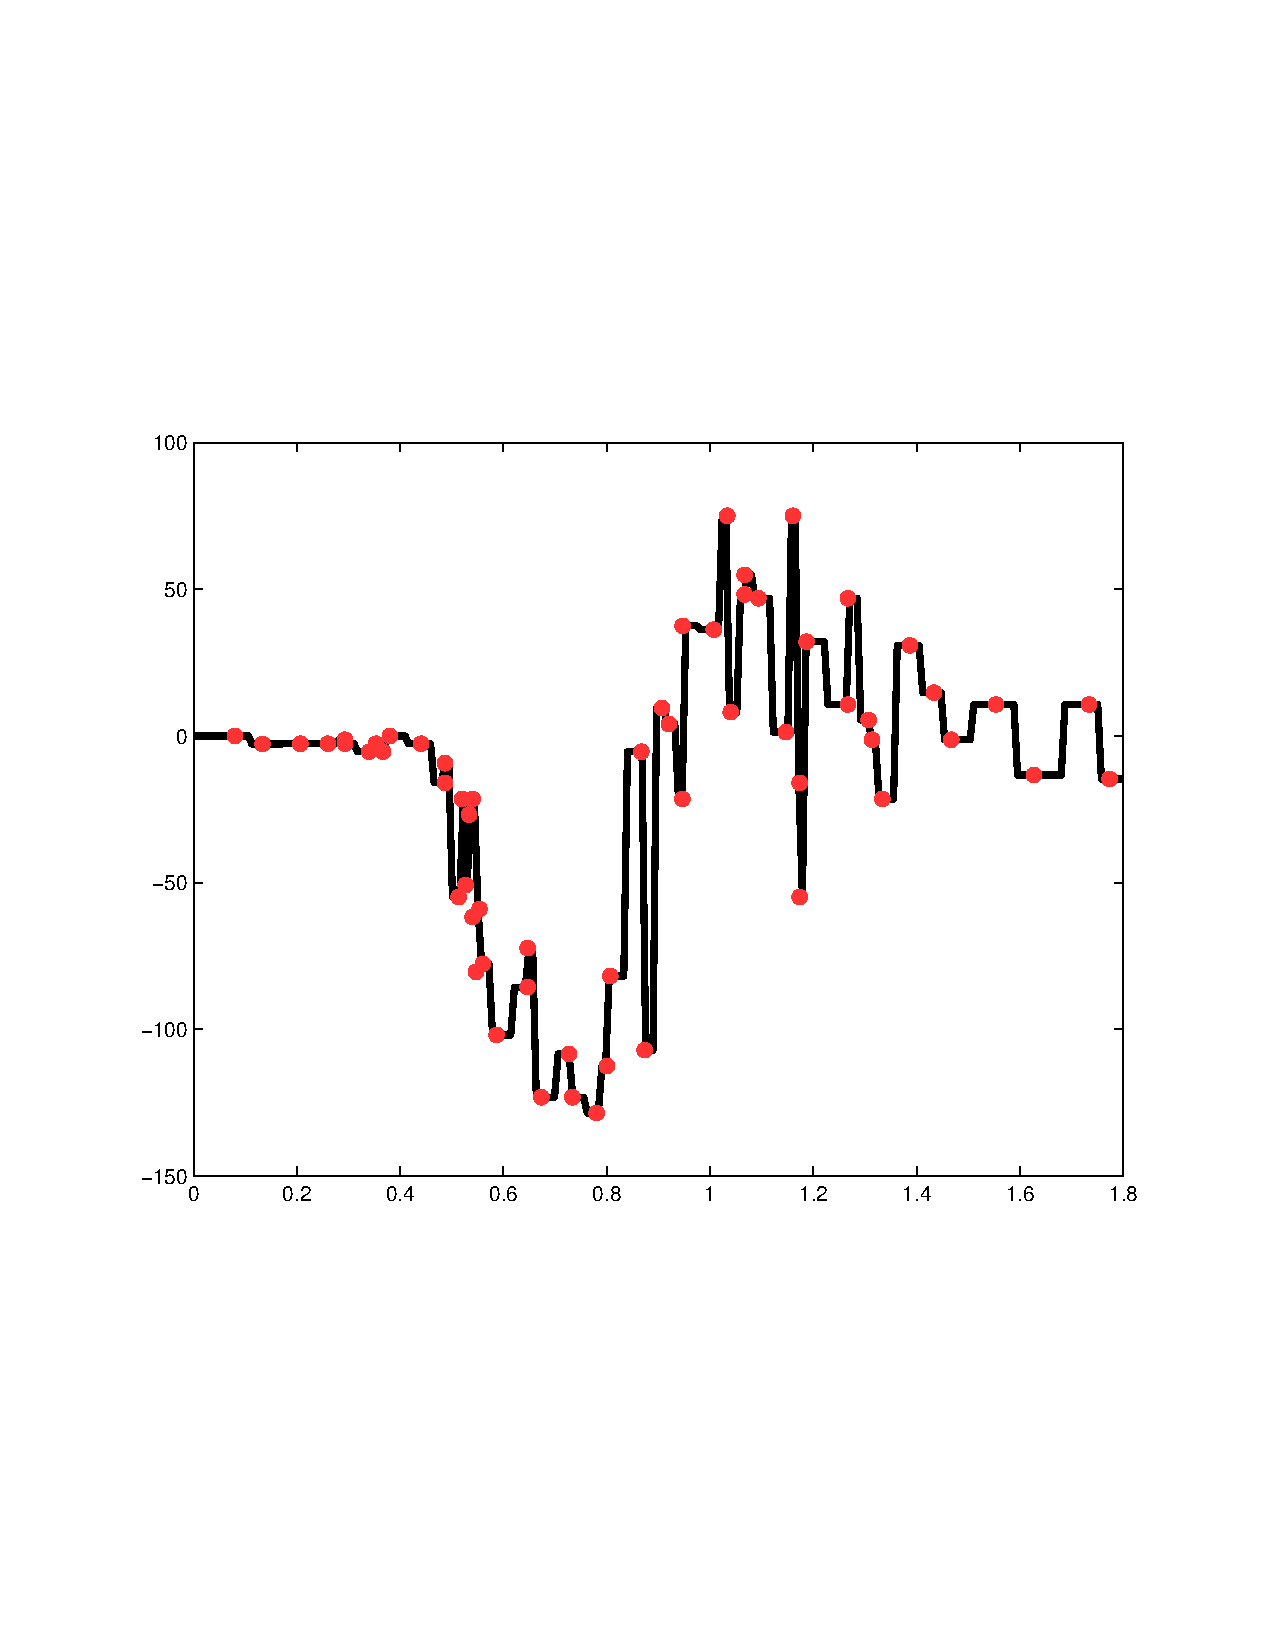
\includegraphics[width=.22\textwidth]{\figdir/problem2_K1} &
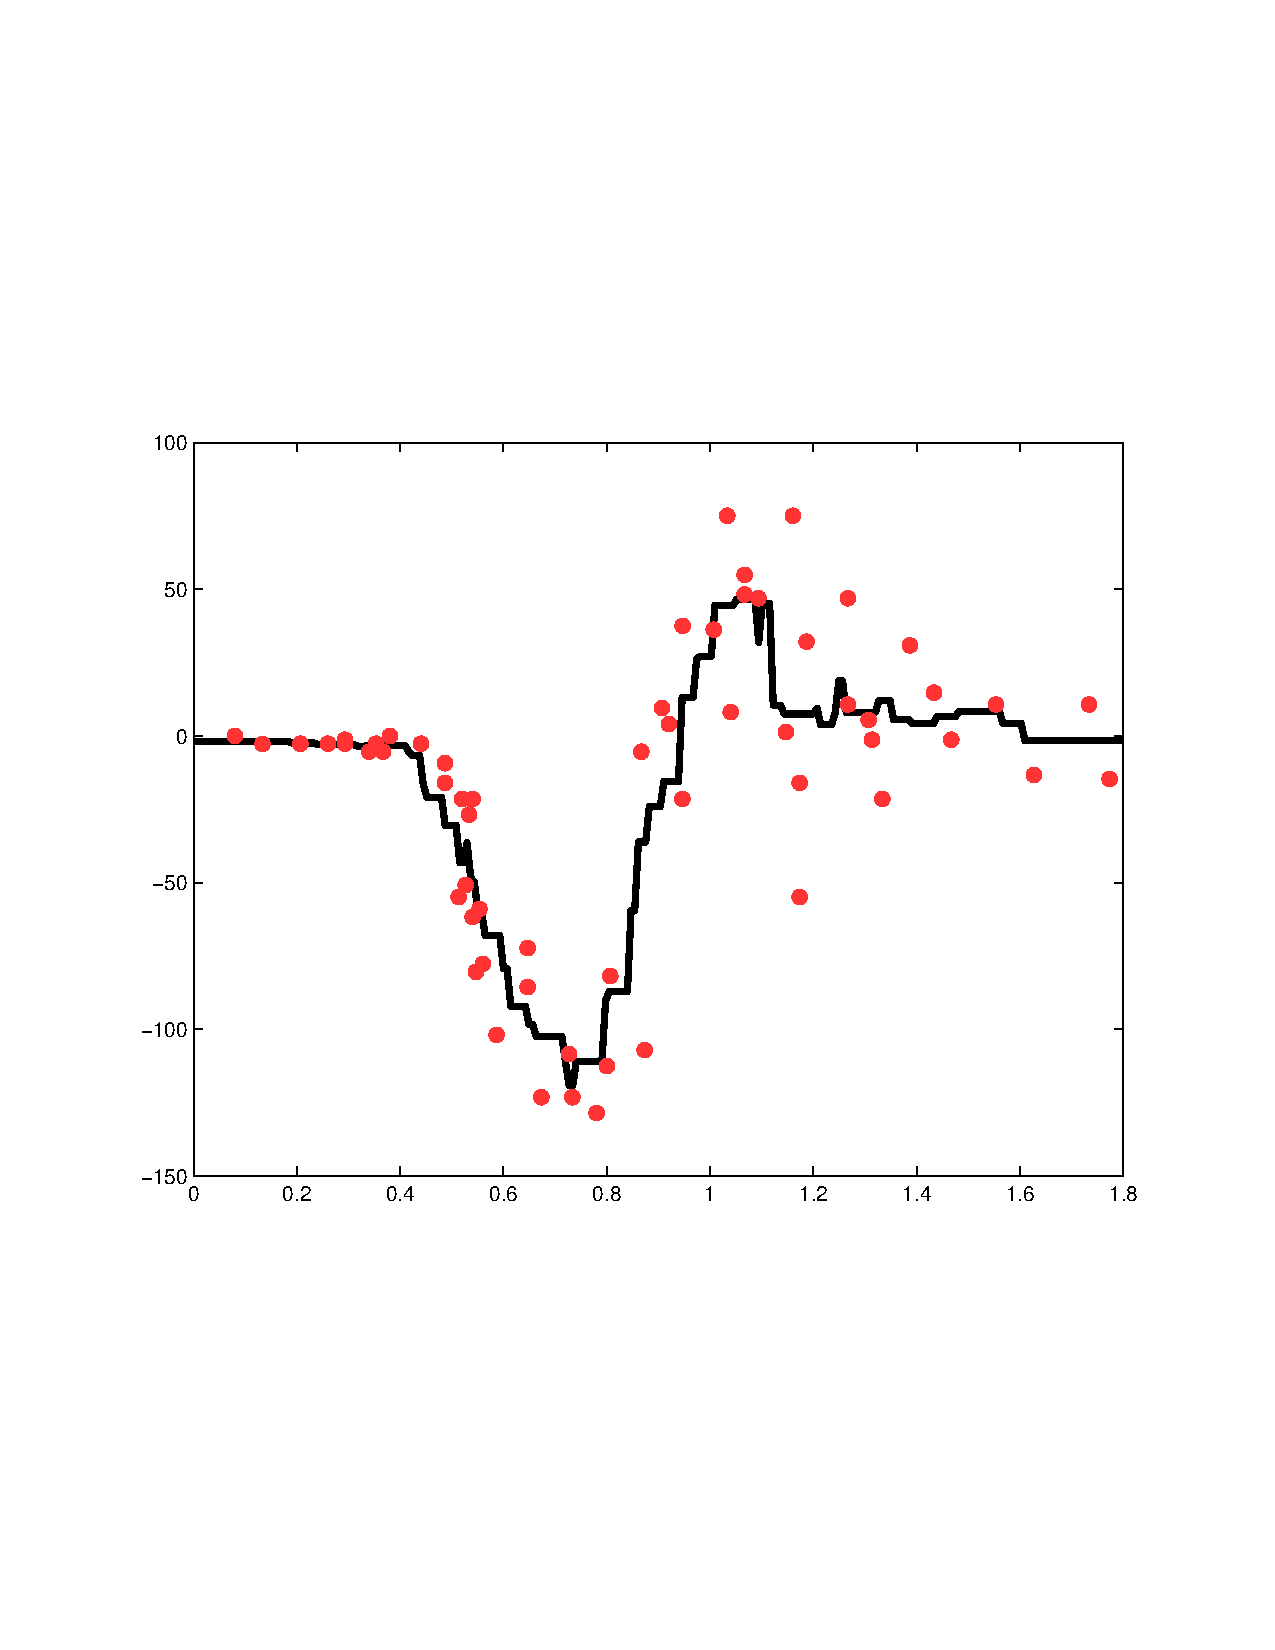
\includegraphics[width=.22\textwidth]{\figdir/problem2_K5} &
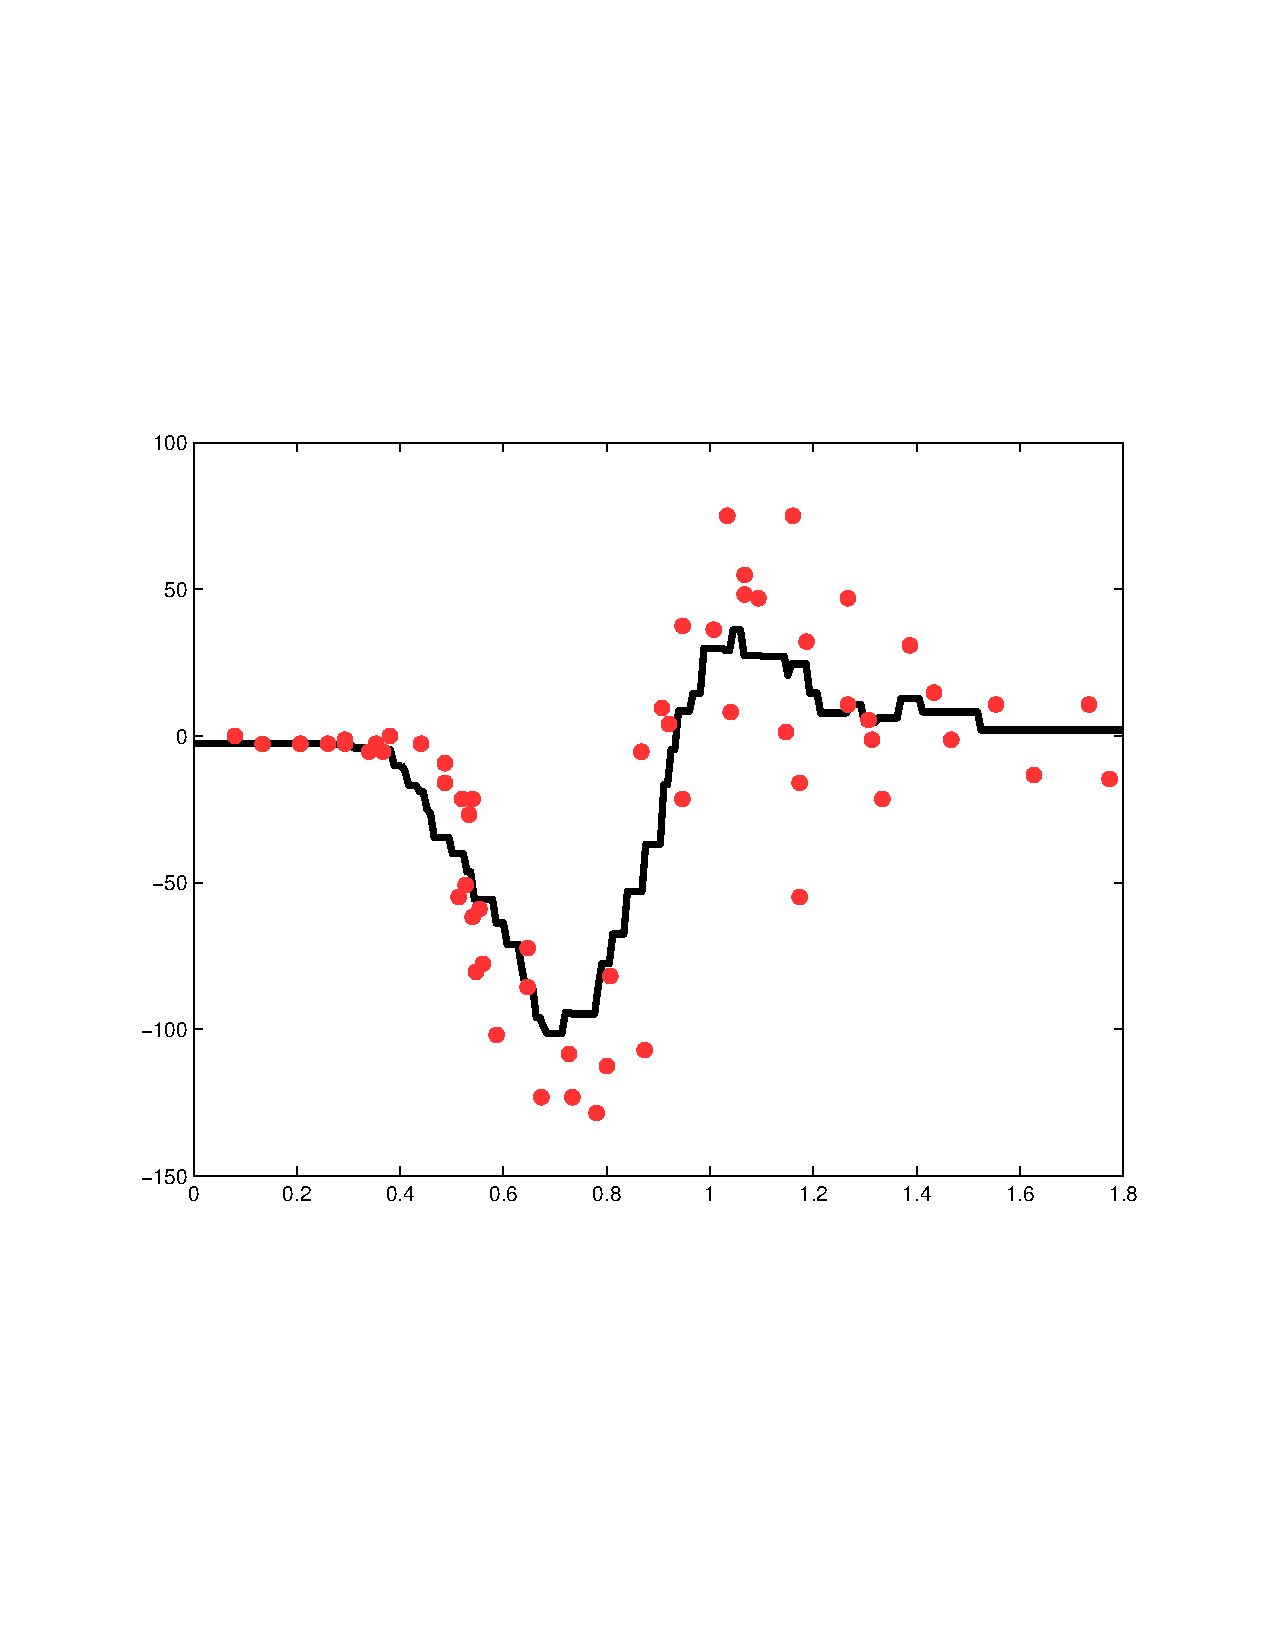
\includegraphics[width=.22\textwidth]{\figdir/problem2_K10} &
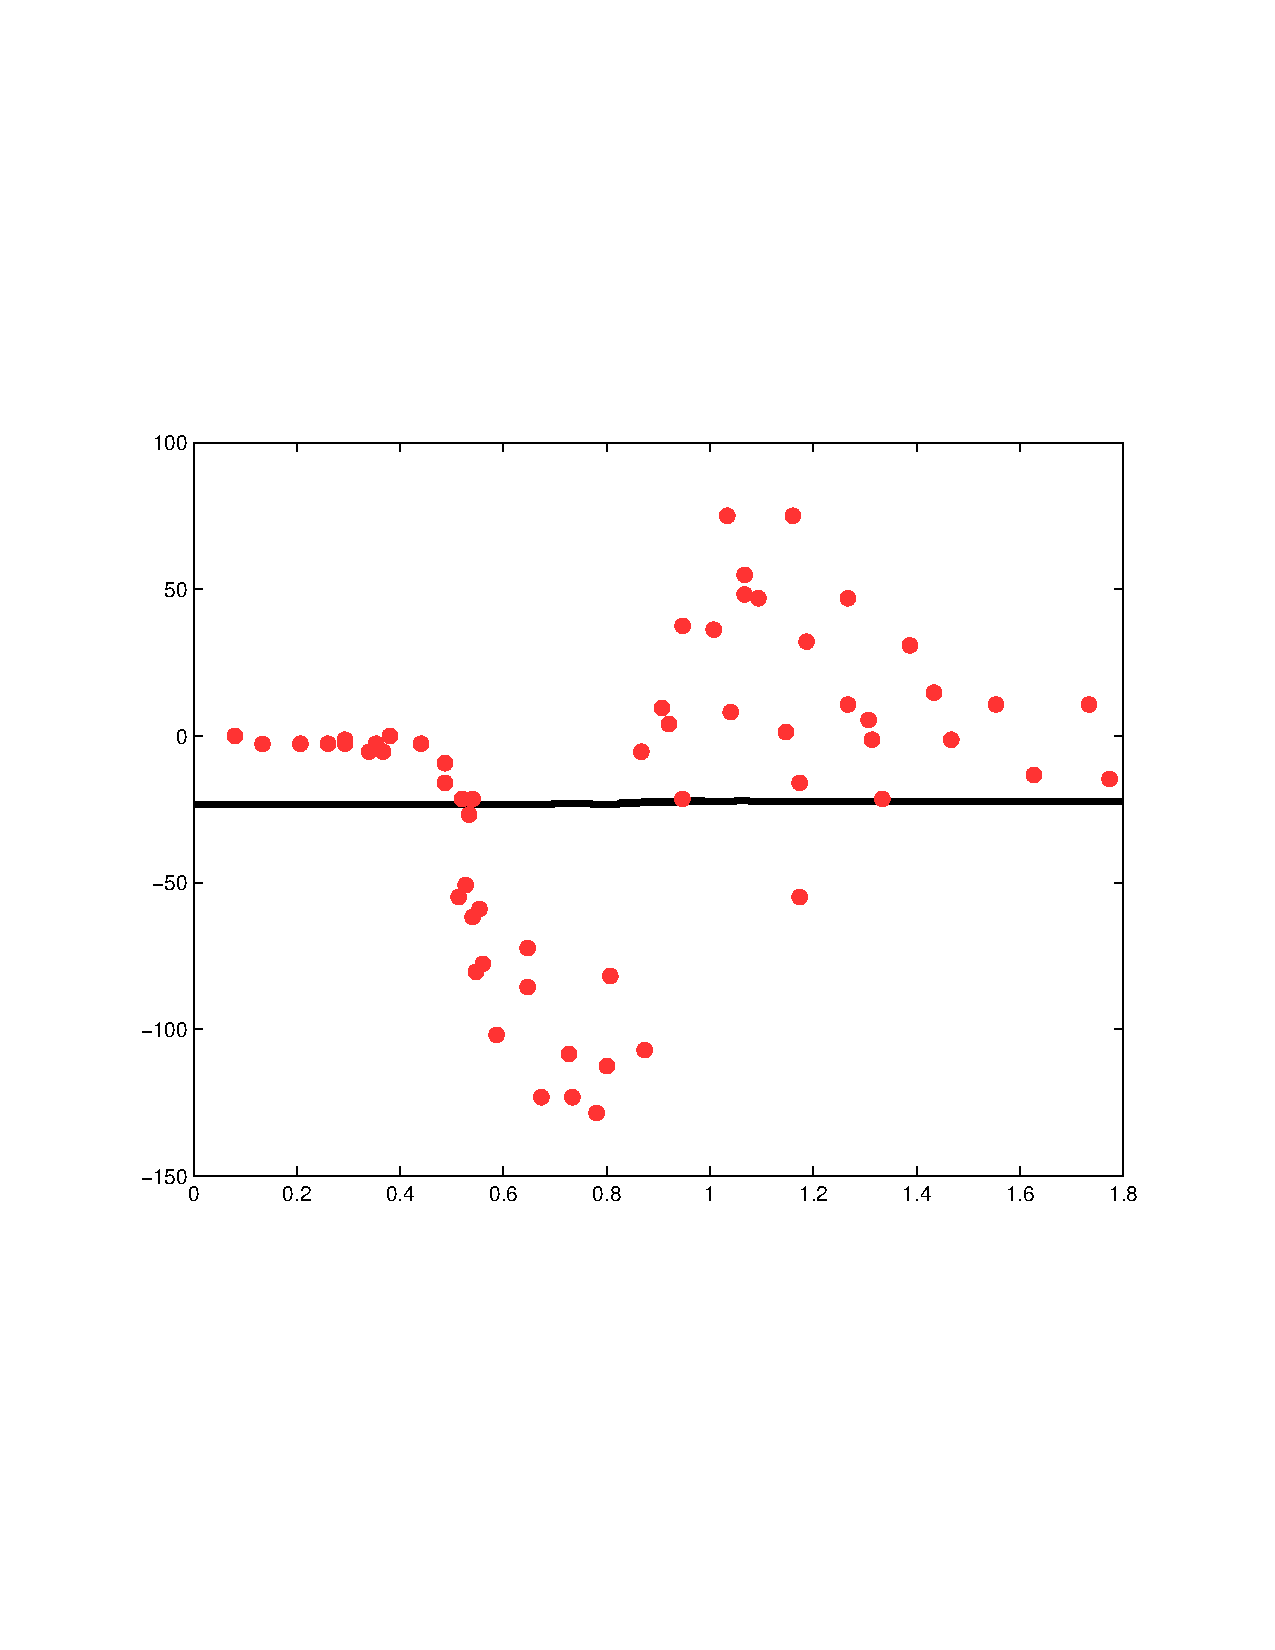
\includegraphics[width=.22\textwidth]{\figdir/problem2_K50} \\
$K=1$ & $K=5$ & $K=10$ & $K=50$ \\
\end{tabular}
\end{figure}

\item 
\begin{figure}[H] \centering
Given the following MSEs: \\
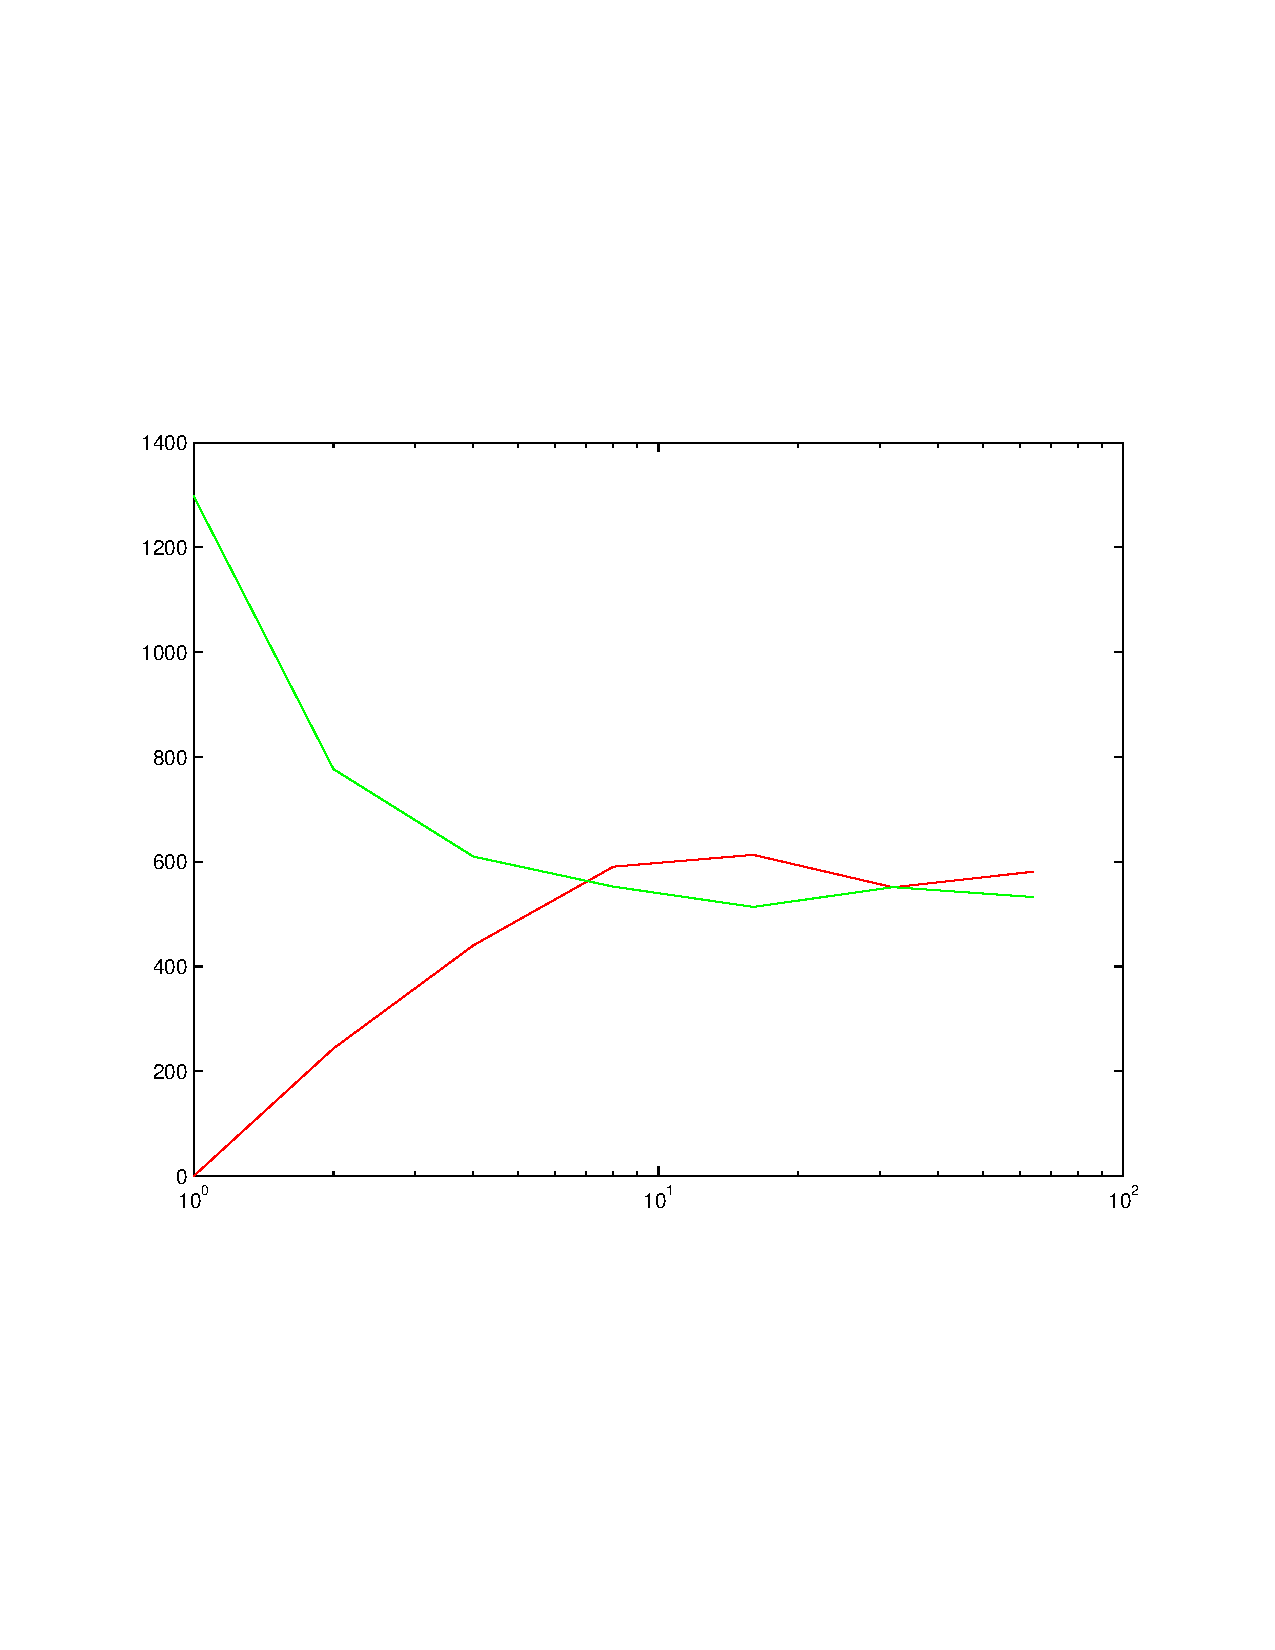
\includegraphics[width=6.5in]{\figdir/prob2b} \\
I would recommend choosing $K=16$ since the MSE appears to increase for the test set after this value.
\end{figure}

\item 
\begin{figure}[H] \centering
Given the following MSEs: \\
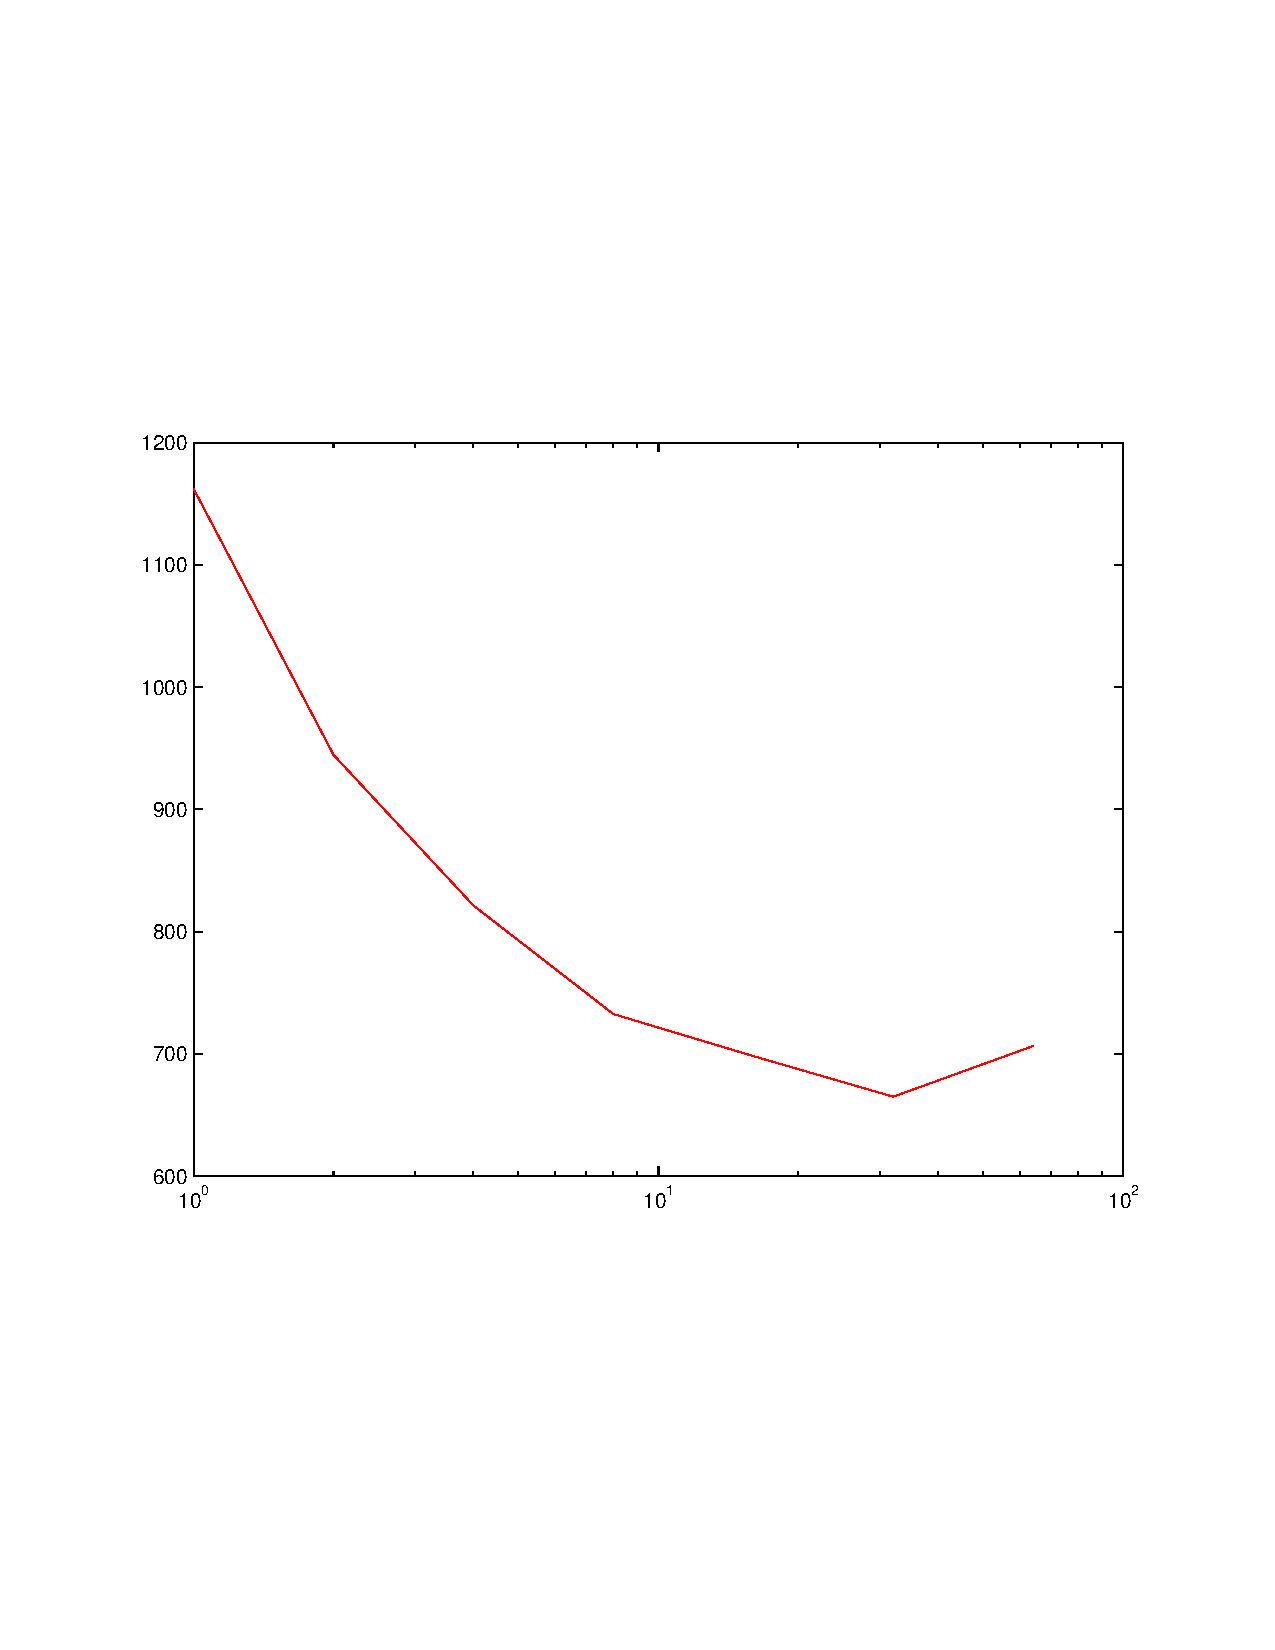
\includegraphics[width=6.5in]{\figdir/prob2c} \\
I would recommend choosing $K=32$ since the MSE appears to increase for the test set after this value.
\end{figure}

\end{enumerate}

% % % % % % % % % % % % % % % % % % % % % % % % % % % % % % % % % % % % % % % % % % % % % % % % % % % % % % % % % % % % % % % %

\subsection*{Problem 3: Bayes Classifiers}

\begin{enumerate}[(a)]
	\item See plot in part c
	\item See plot in part c
	
	\item
		\begin{figure}[H] \centering
		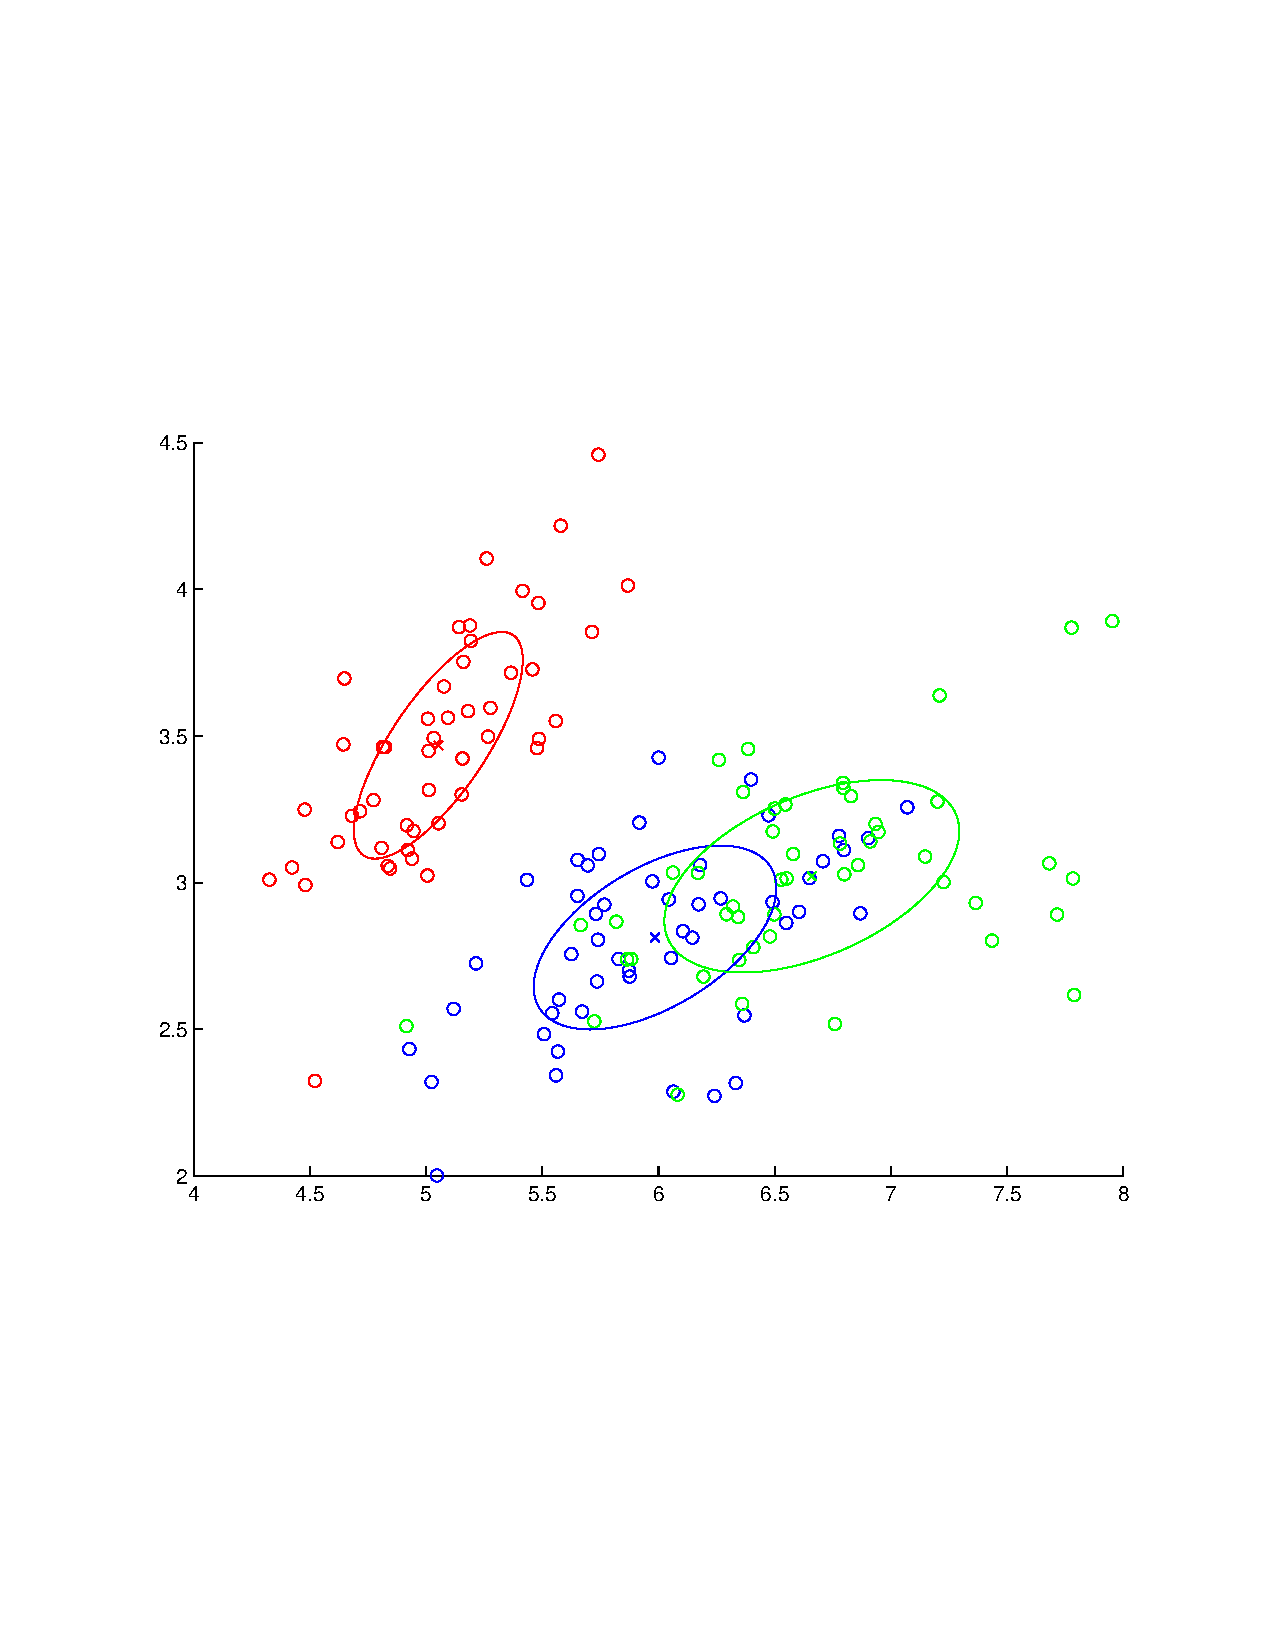
\includegraphics[width=6.5in]{\figdir/prob3a} \\
		\end{figure}
		
	\item
		\begin{figure}[H] \centering
		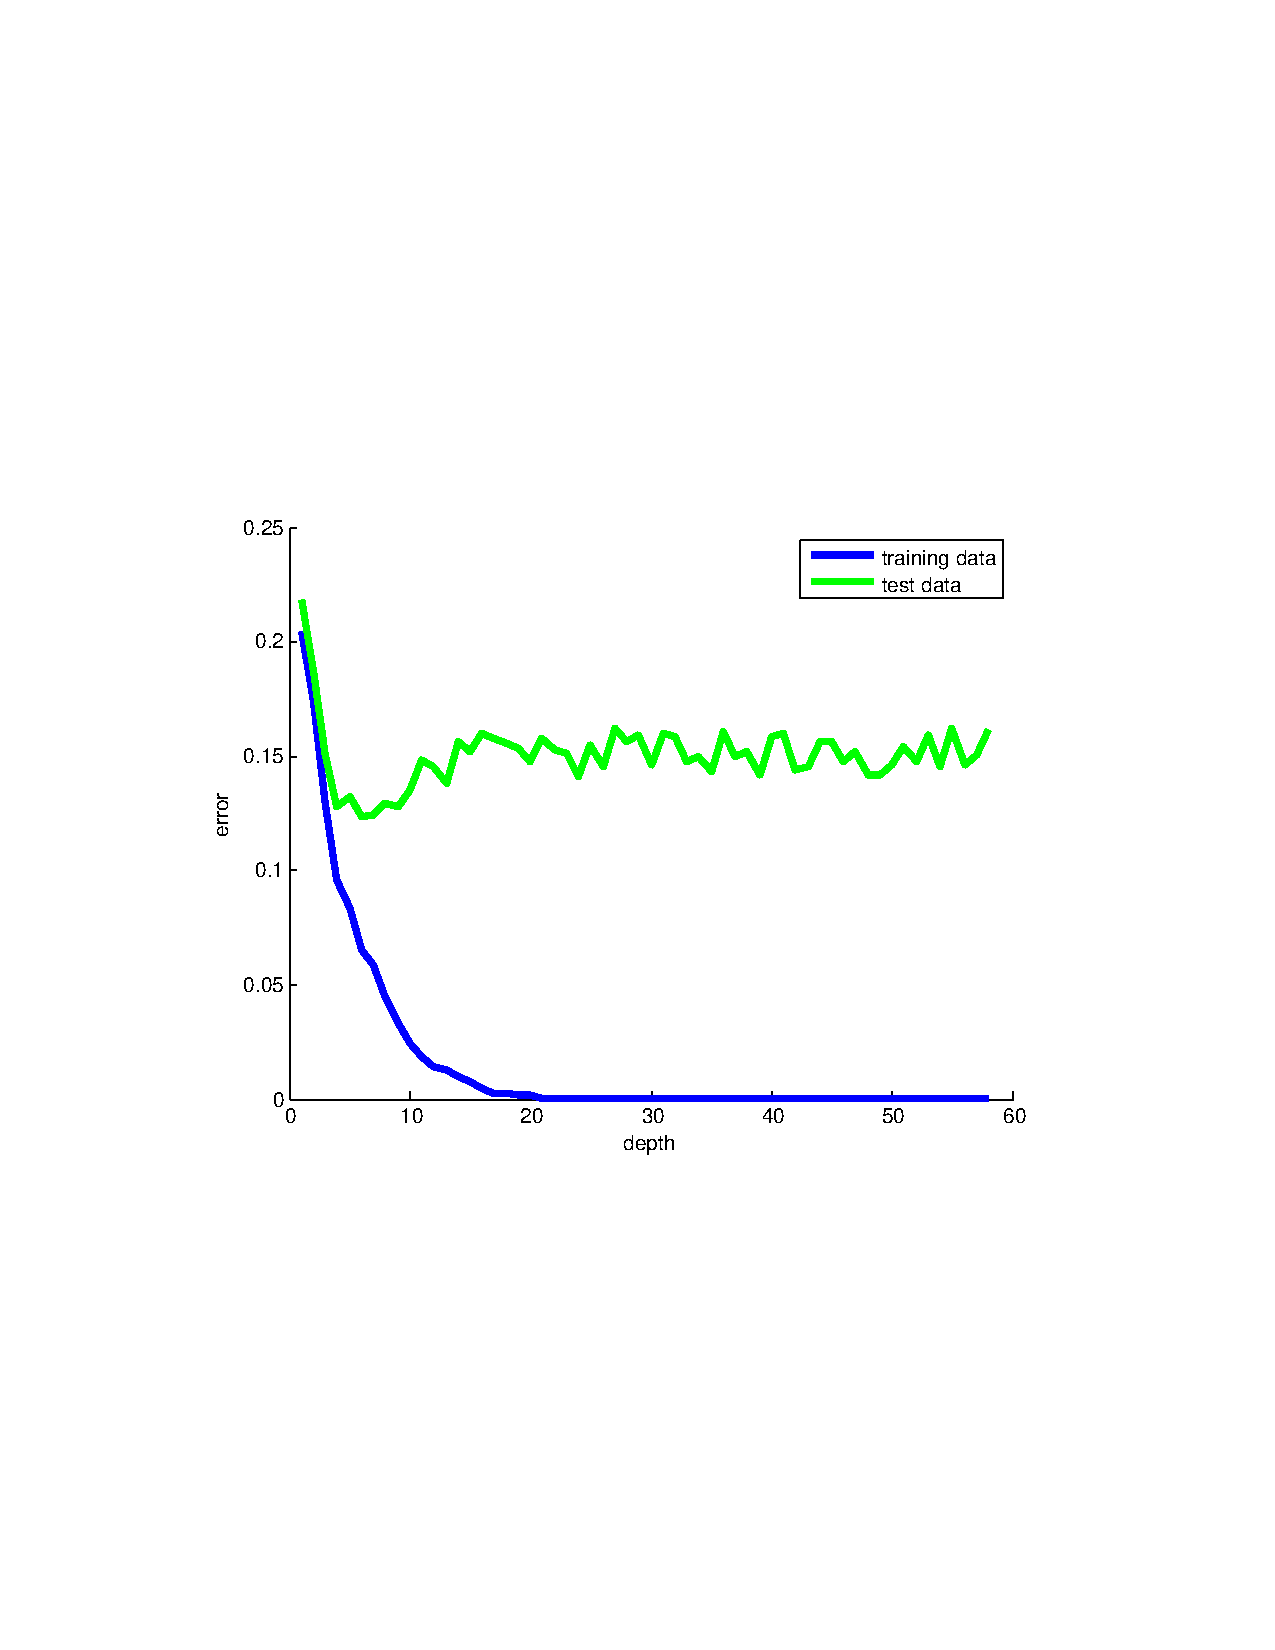
\includegraphics[width=6.5in]{\figdir/prob3b} \\
		\end{figure}

	\item training error rate $=$ 0.2252 \\
		test error rate $=$ 0.5676
	
	\item training error rate $=$ 0.0360 \\
		test error rate $=$ 0.0541
	
\end{enumerate}


% % % % % % % % % % % % % % % % % % % % % % % % % % % % % % % % % % % % % % % % % % % % % % % % % % % % % % % % % % % % % % % %

\subsection*{Problem 4: Decision Trees}

\begin{enumerate}[(a)]
	\item Done
	
	\item
		\begin{figure}[H] \centering
		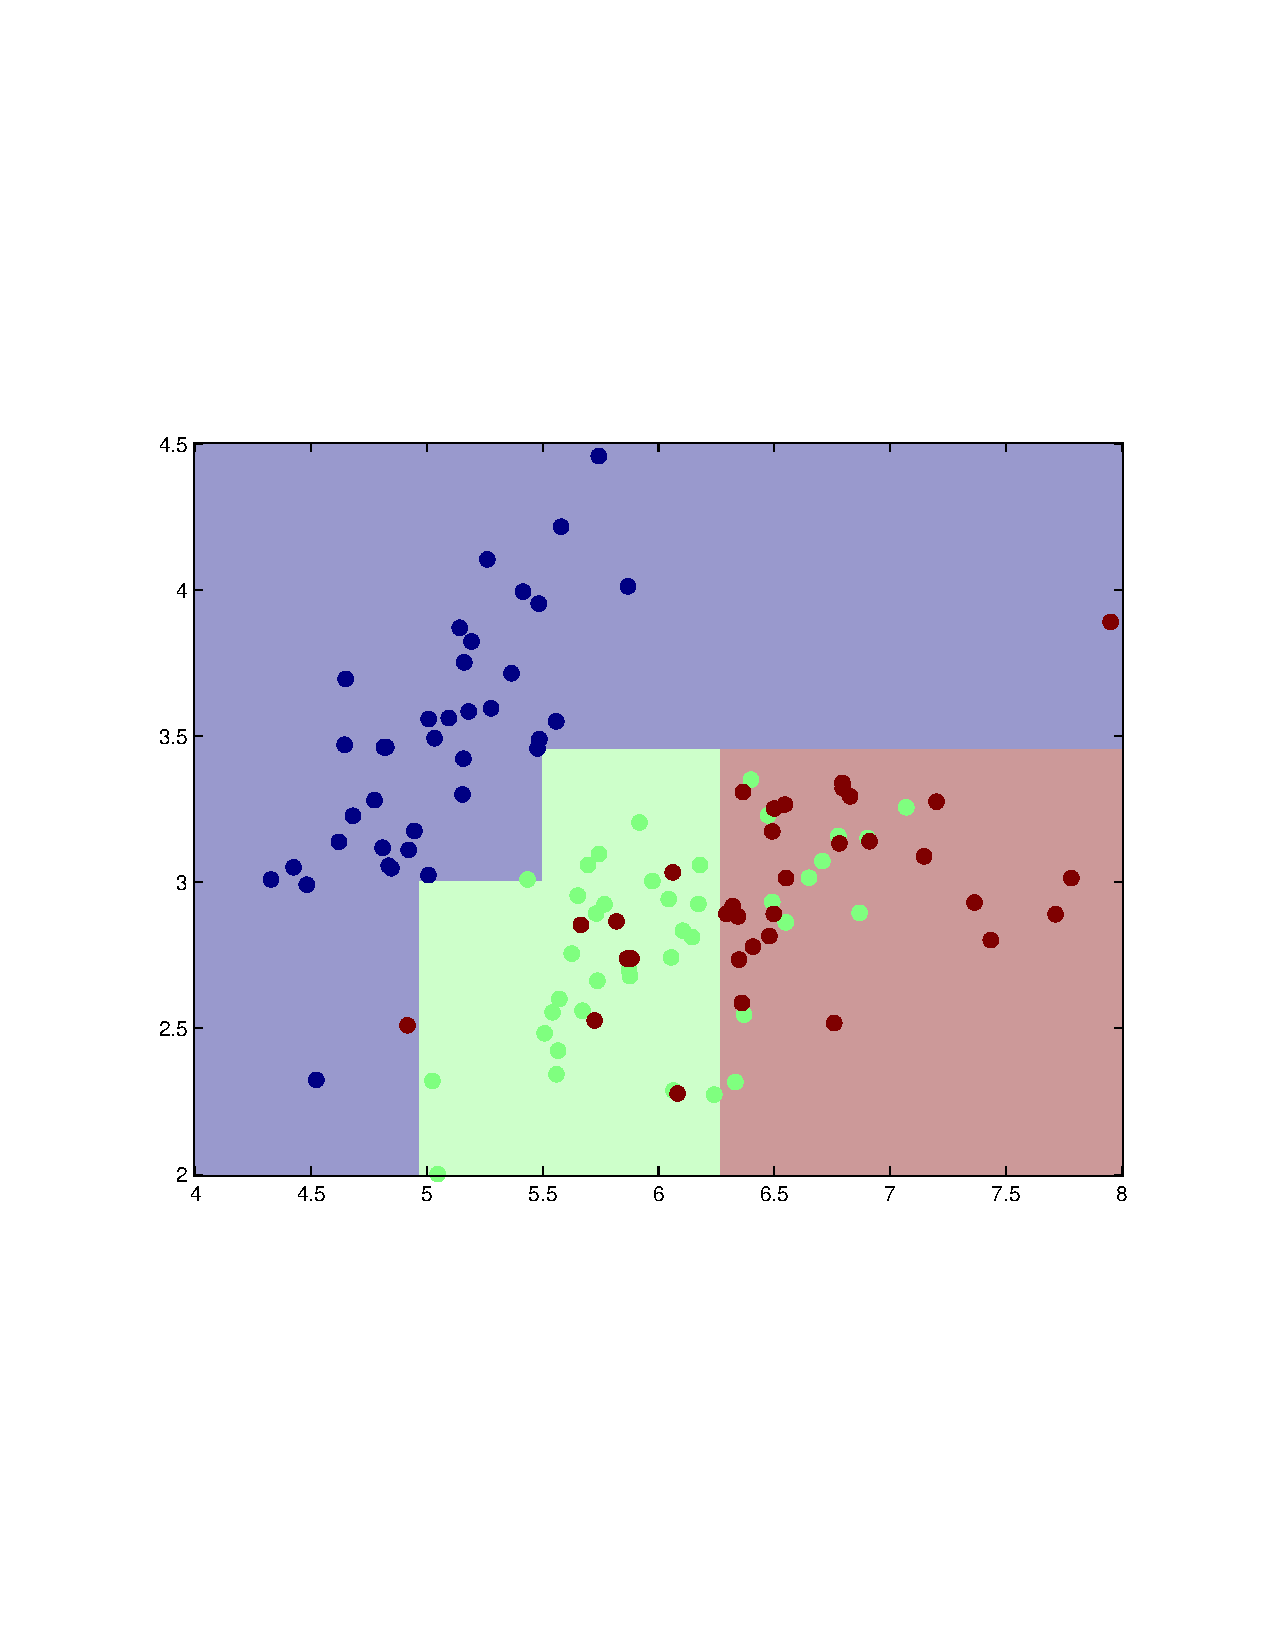
\includegraphics[width=6.5in]{\figdir/prob4} \\
		\end{figure}
		
	\item For 2 features, I would choose to limit the depth to 3.  After several runs, very few seem to improve the misclassification rate beyond a depth of 3 and many runs seem to actually worsen the misclassification rate beyond a depth of 3. Here, the test error comes to around 0.27.

	\item For 4 features, I would choose to limit the depth to 3.  Similarly to the 2 feature case, few runs seem to improve beyond this depth.
Although very few runs actually get worse beyond this depth, many of them show an improvement between depth 2 and 3, so the extra complexity seems to usually be worth it.  Here, the test error comes to between 0 and 0.1.

\end{enumerate}

% % % % % % % % % % % % % % % % % % % % % % % % % % % % % % % % % % % % % % % % % % % % % % % % % % % % % % % % % % % % % % % %

\end{document}
